\section{Construction of Cryptographic Hash Functions}

We discuss two standard methods for constructing
\glsfirstplural{hash function}:
the \MD{} construction and
the sponge construction.
The \MD{} construction is found in many \glspl{hash function} such as
\MDFive{}~\cite{rfc1321}, \ShaOne{}~\cite{FIPS-180-1-1995},
and \ShaTwo{}~\cite{FIPS-180-4-2015}.
The sponge construction is the basis for
\Keccak{}~\cite{KeccakSponge2011}/\ShaThree{}~\cite{FIPS-202}.

\subsection{\MD{} Construction}
\label{app:crypto_md_construction}

The \MD{} construction was described independently 
by Merkle~\cite{merkle1979secrecy}
and Dam\-g\r{a}rd~\cite{damgaard1989design}.
The main idea is to take the long message,
separate the message into blocks,
and operate on those blocks in an iterative fashion.
The hash is then the result of this iterative process.

The construction is built around a \emph{compression function}
$h:\braces{0,1}^{b}\times\braces{0,1}^{n}\to\braces{0,1}^{b}$.
We begin by a discussion of hashing short messages
before we discuss hashing longer messages.
The desired hash output is $b$ bits;
the input message will be split up into blocks of $n$ bits for processing.
The compression function will be used to mix together
the input message.

\subsubsection{Hashing Short Messages}

Let $m\in\braces{0,1}^{n}$ be our message to hash.
We let $\textsf{IV}\in\braces{0,1}^{b}$ be a public
\emph{\gls{initialization vector}}.
We can then define our hash of $m$:

\begin{equation}
    H(m) \mathDef{} h(\textsf{IV}, m).
\end{equation}

\noindent
If $h$ thoroughly scrambles messages, then it should be difficult
to determine $m$ from $H(m)$.

\subsubsection{Hashing Long Messages}

In practice, the messages which need to be hashed may be long;
in particular, they may be longer than $n$ bits.

Let us suppose we have a message $m\in\braces{0,1}^{\ell n}$;
that is, we have

\begin{equation}
    m = m_{0}||m_{1}||\cdots||m_{\ell-1}
\end{equation}

\noindent
with $m_{i}\in\braces{0,1}^{n}$.
We now define the hash of $m$ by an iterative process:

\begin{align}
    h_{0} &= h(\textsf{IV}, m_{0}) \nonumber\\
    h_{1} &= h(h_{0}, m_{1}) \nonumber\\
    h_{2} &= h(h_{1}, m_{2}) \nonumber\\
        &\quad \vdots \nonumber\\
    h_{\ell-1} &= h(h_{\ell-2}, m_{\ell-1}) \nonumber\\
    H(m) &\mathDef{} h_{\ell-1}.
\end{align}

\noindent
In this way, we iteratively mix the entire input together
to obtain the final hash output.

\subsubsection{Message Padding}

At this point, we have always assumed that our messages
have been multiples of $n$-bits;
this will not always be the case in practice.
Thus, \glspl{hash function} take a message as input,
\emph{pad} the message,
and then hash the padded message.
Within the padding, it is common to include the message length.
Including the message length will ensure that messages
of different lengths will \emph{always} result in different padded messages.
Padded messages will always have the following form:

\begin{equation}
    \textsf{pad}(m) = m_{0}||m_{1}||\cdots||m_{\ell-1}.
\end{equation}

\noindent
Here, the appropriate padding scheme ensures that
$m_{i}\in\braces{0,1}^{n}$.

For a general message $m$, we have

\begin{align}
    \textsf{pad}(m) &= m_{0}||m_{1}||\cdots||m_{\ell-1} \nonumber\\
    h_{0} &= h(\textsf{IV}, m_{0}) \nonumber\\
    h_{1} &= h(h_{0}, m_{1}) \nonumber\\
    h_{2} &= h(h_{1}, m_{2}) \nonumber\\
        &\quad \vdots \nonumber\\
    h_{\ell-1} &= h(h_{\ell-2}, m_{\ell-1}) \nonumber\\
    H(m) &\mathDef{} h_{\ell-1}.
\end{align}

\noindent
See Figure~\ref{fig:md_construction} for a graphical representation;
see Alg.~\ref{alg:md_construction} for the specification.

\begin{figure}[t]
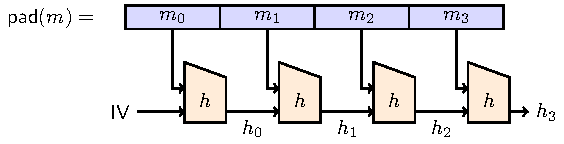
\includegraphics[width=\textwidth]{figures/app_crypto/merkle-damgard/merkle-damgaard.pdf}
\caption[Cryptographic hash function built with \MD{} construction]{Here
    is an example of the \MD{} construction.
    Based on a diagram from~\cite{TikZ:for:Cryptographers}.
    The message is padded so that it is a multiple of the block size.
    After this, the compression function $h$ iteratively processes
    the message blocks.}
\label{fig:md_construction}
\end{figure}

\begin{algorithm}[t]
\caption{Merkle-Damg\r{a}rd construction of hash functions}
\label{alg:md_construction}
\begin{algorithmic}[1]
\Procedure{\MD{}}{$m$}
    \State $m_{0}\|m_{1}\|\cdots\|m_{k-1} \algAssign{} \textsf{pad}(m)$
    \Comment{Pad $m$ appropriately}
    \State $h_{0} \algAssign{} h(\textsf{IV}, m_{0})$
    \Comment{\textsf{IV} is the \gls{initialization vector}}
    \For{$i=1$; $i<k$; $i{+}{+}$}
        \State $h_{i} \algAssign{} h(h_{i-1}, m_{i})$
    \EndFor
    \State \Return $h_{k-1}$
\EndProcedure
\end{algorithmic}
\end{algorithm}


With the particular message padding, there is usually some large
but finite bound on the size of the message.
In particular, \MDFive{}, \ShaOne{}, and \ShaTwo{}-256 
all have a maximum message length of $2^{64}-1$ bits;
\ShaTwo{}-512 has a maximum message length of $2^{128}-1$ bits.
This message length restriction results from the particulars
of the padding process.

To put this length restriction in context,
we note that $2^{64}$ bits is $2^{61}$ bytes or 2 exbibytes.
One terabyte of data ($10^{12}$) is essentially one tebibyte ($2^{40}$);
thus, the message length is limited to approximately
one million terabytes.

\subsubsection{Internal State and Length Extension Attacks}

We will now discuss length extension attacks and how they affect
\glspl{hash function} based on the \MD{} construction.

Suppose we are given $\text{len}(x)$ and $H(x)$.
That is, we are told the length of the unpadded message $x$ and its digest,
but not the message itself.
Then for any message $y$, we can easily compute $H(\textsf{pad}(x)||y)$.

First, we suppose that

\begin{equation}
    \textsf{pad}(x) = x_{0}||x_{1}||\cdots||x_{\ell-1}.
\end{equation}

\noindent
The iterative process tells us that

\begin{align}
    h_{0} &= h(\textsf{IV}, x_{0}) \nonumber\\
        &\quad \vdots \nonumber\\
    h_{\ell-1} &= h(h_{\ell-2}, x_{\ell-1}) \nonumber\\
    H(x) &\mathDef{} h_{\ell-1}.
\end{align}

\noindent
Now, we do not know about $x_{i}$ but we \emph{do know} $H(x) = h_{\ell-1}$;
this is the \emph{entire} internal state of the \gls{hash function} once we
have finished processing $\textsf{pad}(x)$.
We also know

\begin{equation}
    \textsf{pad}\parens{\textsf{pad}(x)||y} = 
        x_{0}||x_{1}||\cdots||x_{\ell-1}||y_{0}||y_{1}||\cdots||y_{k-1}.
\end{equation}

The explicit way to compute $H(\textsf{pad}(x)||y)$ would be
the following:

\begin{align}
    h_{0} &= h(\textsf{IV}, x_{0}) \nonumber\\
        &\quad \vdots \nonumber\\
    h_{\ell-1} &= h(h_{\ell-2}, x_{\ell-1}) \nonumber\\
    h_{\ell} &= h(h_{\ell-1}, y_{0}) \nonumber\\
        &\quad \vdots \nonumber\\
    h_{\ell+k-2} &= h(h_{\ell+k-3}, y_{k-1}) \nonumber\\
    H(\textsf{pad}(x)||y) &\mathDef{} h_{\ell+k-2}.
\end{align}

\noindent
But because we have $H(x) = h_{\ell-1}$, we can instead compute
$H(\textsf{pad}(x)||y)$ by

\begin{align}
    h_{\ell} &= h(h_{\ell-1}, y_{0}) \nonumber\\
    h_{\ell+1} &= h(h_{\ell}, y_{1}) \nonumber\\
        &\quad \vdots \nonumber\\
    h_{\ell+k-2} &= h(h_{\ell+k-3}, y_{k-1}) \nonumber\\
    H(\textsf{pad}(x)||y) &\mathDef{} h_{\ell+k-2}.
\end{align}

\noindent
From our discussion about properties of \glspl{random oracle},
$H(\textsf{pad}(x)||y)$ should always be independent of $H(x)$
(even though $\textsf{pad}(x) = x||z$ for some $z$),
and the only way to learn $H(\textsf{pad}(x)||y)$ should be to explicitly
query the \gls{random oracle}.
We see this is not the case for the \MD{} construction.

Length extension attacks only affect those \glspl{hash function} which output
the entire internal state;
as mentioned, these include \MDFive{}, \ShaOne{}, \ShaTwo{}-256,
and \ShaTwo{}-512.
This \emph{does not} affect \ShaTwo{}-512/224 or \ShaTwo{}-512/256;
in both cases, the 512 bit internal state is truncated
to 224 or 256 bits.
In this way, the entire internal state is not learned,
so this attack fails.

\subsubsection{Example \MD{} Parameters}

We now list the parameters used in
some standard \MD{}-based \glspl{hash function};
see Table~\ref{table:hash_functions}.
The block size of \MDFive{}, \ShaOne{}, and \ShaTwo{}-256
is 512 bits while the internal state and output size
are equal (128, 160, and 256 bits, respectively).
In the case of \ShaTwo{}-512, the block size is 1024 bits
while the internal state and output size is 512 bits.

\begin{table}[t]
\centering
\begin{tabular}{c|c|c|c|c}
\hline
\multicolumn{2}{c|}{\thead{Algorithm and \\ Variant}} &
\thead{Internal State \\ (bits)} &
\thead{Output Size \\ (bits)} &
\thead{Block Size \\ (bits)} \\
\hline
\multicolumn{2}{c|}{\MDFive{}} & 128 & 128 & 512 \\
\hline
\multicolumn{2}{c|}{\ShaOne{}} & 160 & 160 & 512 \\
\hline
\multirow{2}{*}{\ShaTwo{}} & \ShaTwo{}-256 & 256 & 256 & 512 \\
& \ShaTwo{}-512 & 512 & 512 & 1024 \\
\hline
\multirow{2}{*}{\ShaThree{}} & \ShaThree{}-256 & 1600 & 256 & 1088 \\
& \ShaThree{}-512 & 1600 & 512 & 576 \\
\hline
\end{tabular}
\caption[Comparison of Cryptographic Hash Functions]{Comparison
    of various \glsfirstplural{hash function}.
    We know that \MDFive{}, \ShaOne{}, and \ShaTwo{}
    are all based on the \MD{} construction;
    thus, their internal state and output size are the same.
    \ShaThree{} is based on sponge functions;
    its internal state is 1600 bits;
    the block size (rate) depends on the output.
    In the case of \ShaThree{}-256, the capacity is $512=2\cdot256$
    while the rate is $1088 = 1600-512$;
    for \ShaThree{}-512, the capacity is $1024=2\cdot512$
    while the rate is $576 = 1600-1024$.
    This table is based on the table from
    information from~\cite{rfc1321}, \cite[Figure 1]{FIPS-180-4-2015},
    and \cite[Section 6.1]{FIPS-202}.
}
\label{table:hash_functions}
\end{table}



\subsection{Sponge Construction}
\label{app:crypto_sponge_construction}

Attacks on \MDFive{} and \ShaOne{} led to the
\emph{NIST hash function competition} in an effort to design
a more secure \gls{hash function}.
One of the requirements was that all submitted \glspl{hash function}
must not be susceptible to length extension attacks.

\subsubsection{Sponge Function}

The winner of the competition was \Keccak{}.
These functions are based on \emph{sponge functions}.
This requires a random \gls{permutation}
$f:\braces{0,1}^{b}\to\braces{0,1}^{b}$.
Here, we have integers $r + c = b$ with $r,c\ge1$;
$r$ is called the \emph{rate}
and $c$ is called the \emph{capacity}.
The input message $m$ is padded and split into multiples of $r$ blocks.
These blocks are ``absorbed'' into the sponge.
After all the blocks have been absorbed,
the desired number of output bits are ``squeezed'' out.
See Figure~\ref{fig:sponge_construction} for a graphical representation;
see Alg.~\ref{alg:sponge_construction} for the specification.
\ShaThree{} is an official \gls{hash function} for the NIST standard;
NIST modified the original padding scheme from \Keccak{}.

\begin{figure}[p]
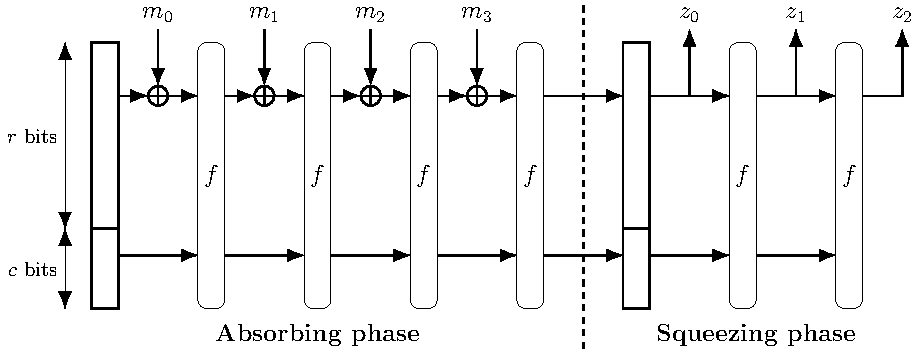
\includegraphics[width=\textwidth]{figures/app_crypto/sponge/sponge.pdf}
\caption[Cryptographic hash function built with Sponge construction]{Here
    is an example of the sponge construction.
    Based on a diagram from~\cite{TikZ:for:Cryptographers}.
    Here, the message $m$ is first padded so that its total length
    is a multiple of the rate $r$.
    The sponge then absorbs the message into its internal state.
    After this, the desired output is squeezed out.}
\label{fig:sponge_construction}
\end{figure}

\begin{algorithm}[p]
\caption{Sponge construction of hash functions;
    based on~\cite[Alg.~1]{KeccakSponge2011}}
\label{alg:sponge_construction}
\begin{algorithmic}[1]
\Require $r < b$
\Procedure{Sponge}{$m$, $\ell$}
    \State $m_{0}\|m_{1}\|\cdots\|m_{k-1} \algAssign{} \textsf{pad}(m, r)$
    \Comment{Pad $m$ to a multiple of $r$}
    \State $s \algAssign{} 0^{b}$
    \Comment{$s$ is initialized to $b$ zero bits}
    \For{$i=0$; $i<k$; $i{+}{+}$}
        \Comment{Absorbing Phase}
        \State $s \algAssign{} s \oplus (m_{i}\|0^{b-r})$
        \State $s \algAssign{} f(s)$
    \EndFor
    \State $z \algAssign{} \textsf{trunc}(s, r)$
    \Comment{Squeezing Phase}
    \While{$\text{len}(z) < \ell$}
        \State $s \algAssign{} f(s)$
        \State $z \algAssign{} z\|\textsf{trunc}(s, r)$
    \EndWhile
    \State \Return $\textsf{trunc}(z, \ell)$
\EndProcedure
\end{algorithmic}
\end{algorithm}


More formally, we first pad the message to a multiple of the rate
with the appropriate padding scheme:

\begin{equation}
    \textsf{pad}(m) = m_{0}||m_{1}||\cdots||m_{k-1}.
\end{equation}

\noindent
Here, we have $m_{i}\in\braces{0,1}^{r}$.
We then absorb the message into the internal state of the sponge:

\begin{align}
    s_{0} &= 0^{b}
        \nonumber\\
    \hat{s}_{0} &= s_{0} \oplus \parens{m_{0}||0^{b-r}}
        \nonumber\\
    s_{1} &= f(\hat{s}_{0})
        \nonumber\\
    \hat{s}_{1} &= s_{1} \oplus \parens{m_{1}||0^{b-r}}
        \nonumber\\
    &\quad \vdots
        \nonumber\\
    \hat{s}_{k-1} &= s_{k-2} \oplus \parens{m_{k-1}||0^{b-r}}
        \nonumber\\
    s_{k} &= f(\hat{s}_{k-1})
\end{align}

\noindent
Here, $0^{b}$ and $0^{b-r}$ mean $b$ zero bits and $b-r$ zero bits,
respectively.
At this point, the sponge has completed the absorbing phase.
We need to squeeze the sponge to produce the desired output.
If $\ell$ bits of output are desired with $jr < \ell \le \parens{j+1}r$,
then compute

\begin{align}
    z_{0} &= \textsf{trunc}(s_{k}, r)
        \nonumber\\
    s_{k+1} &= f(s_{k})
        \nonumber\\
    z_{1} &= \textsf{trunc}(s_{k+1}, r)
        \nonumber\\
    s_{k+2} &= f(s_{k+1})
        \nonumber\\
    &\quad \vdots
        \nonumber\\
    z_{j} &= \textsf{trunc}(s_{k+j}, r)
        \nonumber\\
    z &= \textsf{trunc}(z_{0}||z_{1}||\cdots||z_{j}, \ell)
        \nonumber\\
    H(m) &\mathDef{} z.
\end{align}

\noindent
Here, \textsf{trunc} refers to returning the
specified number of bits.
This defines the output of a \gls{hash function} based
on the sponge construction.

\subsubsection{Sponge Function Security}

For a given internal state $b$, there is a tradeoff
between rate and capacity.
A larger rate leads to faster computation
because there are fewer blocks to process.
A larger capacity gives the sponge greater security
because less information about the internal state is revealed.
Generic attacks against sponge functions use at least
$2^{c/2}$ operations~\cite[Chapter 5]{KeccakSponge2011},
so this gives a lower bound on the capacity.
Thus, if $k$ bits of security is desired,
it would make sense for $c = 2k$.

Due to the fact that the entire internal state is not revealed
during the squeezing phase,
sponge \glspl{hash function} may be made immune to length extension attacks
provided the capacity is large enough;
that is, if the capacity is large enough, the best method is only
brute force.

\subsubsection{Example Sponge Parameters}

We now list the sponge parameters used in
\Keccak{} and \ShaThree{}.

\paragraph{Padding Differences}
\Keccak{} and \ShaThree{} have slightly different padding schemes:

\begin{align}
    \textsf{pad}_{\text{\Keccak{}}}(m) &\mathDef{}
            m||\texttt{10}^{*}\texttt{1} \nonumber\\
        &= m_{0}||m_{1}||\cdots||m_{\ell-1} \nonumber\\
    \textsf{pad}_{\text{\ShaThree{}}}(m) &\mathDef{}
            m||\texttt{0110}^{*}\texttt{1} \nonumber\\
        &= m_{0}||m_{1}||\cdots||m_{\ell-1}.
\end{align}

\noindent
Here, we have $m_{i}\in\braces{0,1}^{r}$, where $r$ is the rate.
The notation $\texttt{0}^{*}$ means that we add zero or more \texttt{0} bits
for the padding scheme.
In the case of \Keccak{}, we input is appended so that the message
length is a multiple of the rate $r$ (examples are discussed next).
Other \ShaThree{} functions have different padding schemes as well.

\paragraph{Rate and Capacity Examples}
A comparison between \glspl{hash function} may be found in
Table~\ref{table:hash_functions}.
Although \Keccak{} is defined for a number of internal states,
\ShaThree{} focuses only on those with internal state $b=1600$ bits,
as this was the primary submission.
We recall that for sponge functions the \emph{block size}
is called the \emph{rate}.
In \ShaThree{}, due to generic attacks, the capacity is twice
the desired security level.
In this way, \ShaThree{}-256 has capacity $512$ and rate $1088$
while \ShaThree{}-512 has capacity $1024$ and rate $576$.
